\documentclass{standalone}


% Copy of relevant parts from the main preamble.
\usepackage{mathtools}

% Uncomment the following to use Times New Roman and Cambria Math
% \usepackage{unicode-math}
% \unimathsetup{math-style=TeX}
% \setmathfont[range=\mathup/{num}]{Times New Roman}
% \setmathfont[range=\mathit/{greek,Greek,latin,Latin}]{Cambria Math}
% \setmathfont[range=\mathup/{greek,Greek,latin,Latin}]{Cambria Math}
% \setmathfont[range={"2212,"002B,"003D,"0028,"0029,"005B,"005D,"221A,
% "2211,"2248,"222B,"007C,"2026,"2202,"00D7,"0302,"2261,"0025,"22C5,
% "00B1,"2194,"21D4,"2032}]
% {Cambria Math}
% \setmainfont[Ligatures=TeX]{Times New Roman}

% Uncomment the following to use Linux Libertine
% \usepackage[libertine]{newtxmath}
% \usepackage[no-math]{fontspec}
% \setmainfont{Linux Libertine O}

% Uncomment the following to use TeX Gyre Termes
% \usepackage{unicode-math}
% \unimathsetup{math-style=TeX}
% \setmainfont{TeX Gyre Termes}
% \setmathfont{TeX Gyre Termes Math}

% Uncomment the following to use TeX Gyre Pagella
\usepackage{unicode-math}
\unimathsetup{math-style=TeX}
\setmainfont{TeX Gyre Pagella}
\setmathfont{TeX Gyre Pagella Math}

% \usepackage[sfmath]{kpfonts}
% \renewcommand*\familydefault{\sfdefault}
% \usepackage[T1]{fontenc}

% \usepackage[no-math]{fontspec}
% Always use Inconsolata
\setmonofont{Inconsolata}

\usepackage{microtype}


\usepackage[version=3]{mhchem}
\usepackage{chemfig}
\setatomsep{2.25em}
\usetikzlibrary{positioning, calc, arrows.meta}
\tikzset{
    flux/.style={
        flux/.cd,
        #1,
        print,
    },
    flux/.cd,
    position/.store in=\position,
    position=0.6,
    fluxabove/.store in=\fluxabove,
    fluxbelow/.store in=\fluxbelow,
    print/.style={
        /tikz/.cd,
        insert path={%
            node [pos=\position, above] {\SI{\fluxabove}{\percent}} node[pos=\position, below] {\textbf{\SI{\fluxbelow}{\percent}}}%
        },
    },
}
\usepackage{siunitx}
\sisetup{detect-all=true}

\begin{document}
    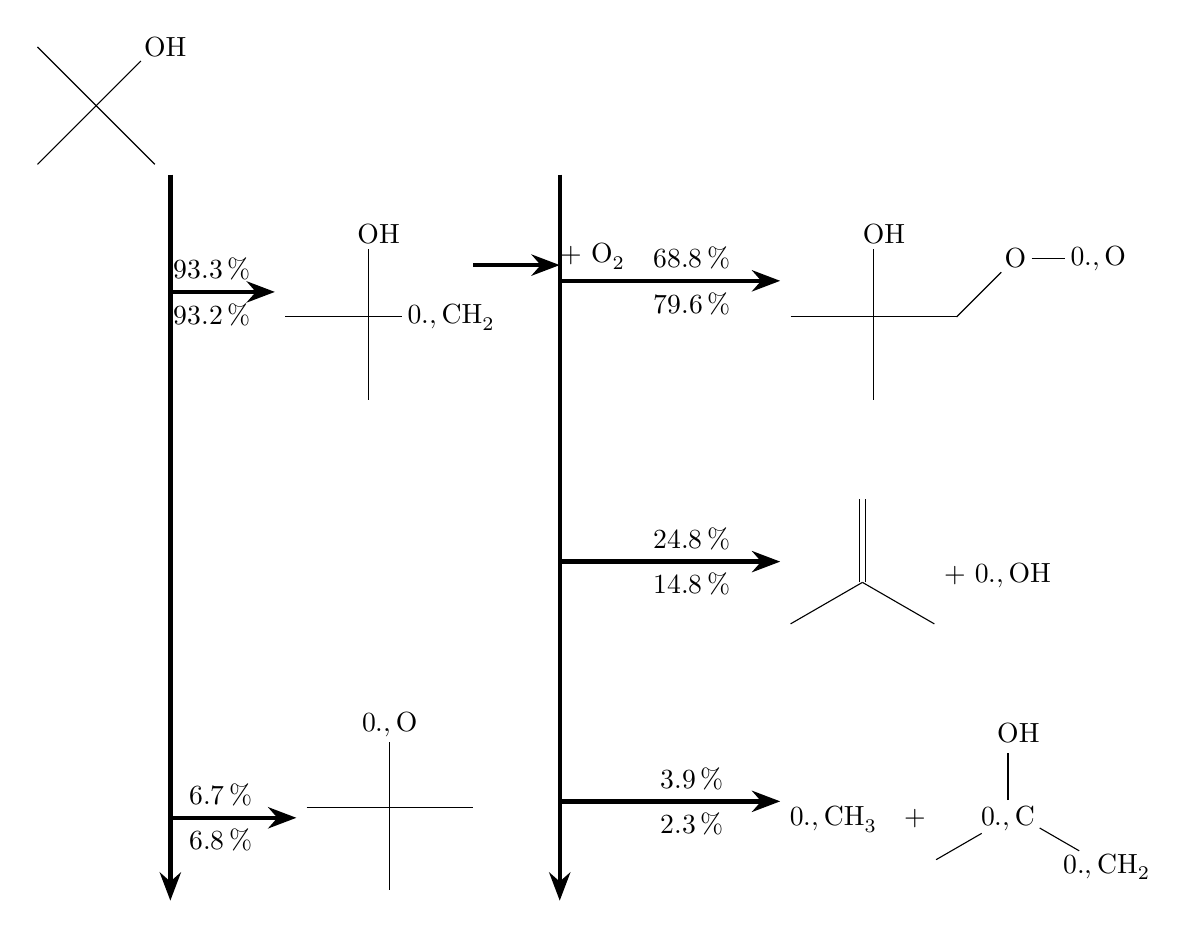
\begin{tikzpicture}[x=1cm, y=1cm, remember picture]
        \begin{scope}
            \node (tbuoh) {\chemfig{[1]-@{center carbon}(-[3])(-[7])-OH}};
            \node[below right=0.5 and 1 of tbuoh] (btbuoh) {\chemfig{-(-[2]OH)(-[6])-\lewis{0.,CH_2}}};
            \node[right=3.5 of btbuoh] (btbuohoo) {\chemfig{-(-[2]OH)(-[6])--[1]O-\lewis{0.,O}}};
            \node[below left=1 and 0 of btbuohoo, anchor=north west] (butene) {\chemfig[baseline=(c)]{-[:30]@{c}(=[2])-[:330]} $+$ \chemfig{\lewis{0.,OH}}};
            \node[below left=1 and 0 of butene, anchor=north west] (scission) {\chemfig{\lewis{0.,CH_3}}\quad $+$ \chemfig[baseline=(d)]{-[:30]\lewis{0.,C}@{d}(-[2]OH)-[:330]\lewis{0.,CH_2}}};
            \node (otbuoh) at (btbuoh |- scission) {\chemfig{-(-[2]\lewis{0.,O})(-[6])-}};
        \end{scope}

        \begin{scope}[every path/.style={draw, ultra thick, >={Stealth}}]
            \path[->] let \p1 = (otbuoh.south), \p2 = (center carbon |- tbuoh.south) in (\x2,\y2) coordinate (linestart) -- (\x2,\y1) coordinate (lineend);
            \path[->] ($(linestart)!(btbuoh.170)!(lineend)$) -- (btbuoh.170) [flux={fluxabove=93.3, fluxbelow=93.2, position=0.4}];
            \path[->] ($(linestart)!(otbuoh.190)!(lineend)$) -- (otbuoh.190) [flux={fluxabove=6.7, fluxbelow=6.8, position=0.4}];
            \coordinate (midline) at ($(btbuoh.east)!0.2!(btbuohoo.west)$);
            \path[->] let \p1 = (linestart), \p2 = (midline), \p3 = (lineend) in (\x2,\y1) -- (\x2,\y3) coordinate (midlineend);
            \path[->] ($(midline)!(btbuohoo.170)!(midlineend)$) -- (btbuohoo.170) node[pos=0.15, above] {$+$ \ce{O2}} [flux={fluxabove=68.8, fluxbelow=79.6}];
            \path[->] ($(midline)!(butene.west)!(midlineend)$) -- (butene.west) [flux={fluxabove=24.8, fluxbelow=14.8}];
            \path[->] ($(midline)!(scission.west)!(midlineend)$) -- (scission.west) [flux={fluxabove=3.9, fluxbelow=2.3}];
            \path[->] let \p1 = ($(btbuoh.east)-(0.4,0)$), \p2 = ($(btbuohoo.170)+(0,0.2)$), \p3 = (midline) in (\x1,\y2) -- (\x3,\y2);
        \end{scope}
    \end{tikzpicture}
\end{document}
